% This must be in the first 5 lines to tell arXiv to use pdfLaTeX, which is strongly recommended.
\pdfoutput=1
% In particular, the hyperref package requires pdfLaTeX in order to break URLs across lines.

\documentclass[11pt]{article}

% Remove the "review" option to generate the final version.
\usepackage[]{ACL2023}

% Standard package includes
\usepackage{times}
\usepackage{latexsym}
\usepackage{booktabs}
\usepackage{graphicx}
\usepackage{subcaption}

% For proper rendering and hyphenation of words containing Latin characters (including in bib files)
\usepackage[T1]{fontenc}
% For Vietnamese characters
% \usepackage[T5]{fontenc}
% See https://www.latex-project.org/help/documentation/encguide.pdf for other character sets

% This assumes your files are encoded as UTF8
\usepackage[utf8]{inputenc}

% This is not strictly necessary, and may be commented out.
% However, it will improve the layout of the manuscript,
% and will typically save some space.
\usepackage{microtype}

% This is also not strictly necessary, and may be commented out.
% However, it will improve the aesthetics of text in
% the typewriter font.
\usepackage{inconsolata}
\usepackage{graphicx}


% If the title and author information does not fit in the area allocated, uncomment the following
%
%\setlength\titlebox{<dim>}
%
% and set <dim> to something 5cm or larger.

\title{Fine-tune of Chemical Language Model}

% Author information can be set in various styles:
% For several authors from the same institution:
% \author{Author 1 \and ... \and Author n \\
%         Address line \\ ... \\ Address line}
% if the names do not fit well on one line use
%         Author 1 \\ {\bf Author 2} \\ ... \\ {\bf Author n} \\
% For authors from different institutions:
% \author{Author 1 \\ Address line \\  ... \\ Address line
%         \And  ... \And
%         Author n \\ Address line \\ ... \\ Address line}
% To start a seperate ``row'' of authors use \AND, as in
% \author{Author 1 \\ Address line \\  ... \\ Address line
%         \AND
%         Author 2 \\ Address line \\ ... \\ Address line \And
%         Author 3 \\ Address line \\ ... \\ Address line}

\author{Faria Alam \\
   7011180 \\\And
   Muhammad Sabeeh Rehman \\
   7047213 \\\And
   Hafiza Hajrah Rehman \\
   7063002 \\}
 

\begin{document}
\maketitle
\begin{abstract}
In this experimental analysis, we fine-tune a chemical LM model Molformer. To enhance it's performance, we explore three experimental strategies. Our results demonstrate that the experiments have increased the model's predictive performance significantly.  
\end{abstract}
\section*{Introduction}
In our project we utilize a transformer-based neural network model from \cite{ross2022largescalechemicallanguagerepresentations} trained on two public chemical datasets PubChem and ZINC in a self-supervised fashion. We use this pre-trained \verb|Molformer model| for our downstream prediction task after fine-tuning it with the \verb|Lipophilicity| dataset. Here, three different type of experiments were done: masked language modeling with the \verb|Lipophilicity| dataset in unsupervised fashion, again fine-tuning the model with the combined dataset of \verb|Lipophilicity| and external influential data samples measured by influence function, applying different data selection techniques and parameter-efficient fine-tuning strategies to improve model's performance.


\section*{Experimental Setup}

\textbf{Data} For the first task the \verb|Lipophilicity| dataset from Hugging face \footnote{\url{https://huggingface.co/datasets/scikit-fingerprints/MoleculeNet_Lipophilicity}} has 4200 samples of sequences of chemical molecules called the \verb|SMILES representation| or \verb|SMILES strings| along with its lipophilicity values which is the target label. The 300 external samples that we use to choose impactful datapoints have a similar structure. Target values for both datasets were normalized to 0-1 using \verb|MinMaxScaler()| 

\textbf{Model} The pre-trained \verb|Molformer model| is used as backbone model and a 2-layer neural network is used as regression head. Output of the \verb|Molformer| model is a compressed mean pool representation of the \verb|SMILES strings| of dimension 768 which is then fed into the regression head. An overview of the pipeline including our downstream regression task is illustrated in this image \ref{fig:pipeline_regression}. In the regression head, we used \verb|Relu| for non-linearity and dropout as a regularizer with 0.1 probability. This is used as the base model for performance comparisons.    

\begin{figure}[htp]
    \centering
    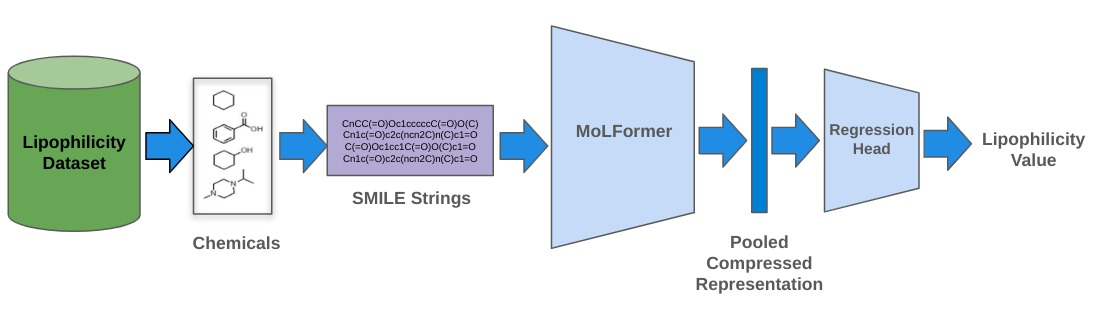
\includegraphics[width=0.5\textwidth]{pictures/pipeline.jpeg}
    \caption{Molformer pipeline with downstream regression head}
    \label{fig:pipeline_regression}
\end{figure}

\textbf{Metrics} For this regression task, our primary metrics are mean squared error(MSE), root mean squared error(RMSE). In addition with these, we also use Spearman, Pearson correlation, R-squared to understand correlation and variability of target label. 

\section*{Fine-tuning Chemical LM on Lipophilicity}
In this first task, we fine-tune our pre-trained \verb|Molformer model| with regression head using \verb|Lipophilicity| dataset to predict the \verb|Lipophilicity| value. Then the same \verb|Molformer model| is fine-tuned in unsupervised manner using \verb|masked language modeling(mlm)| and only \verb|SMILES strings|. In both experiments, the \verb|SMILES strings| are tokenized using \verb|AutoTokenizer| and converted into a vector representation of dimensions 768. We measured all performance metrics on three seed values to ensure reproducibility. The effect of further \verb|masked language modeling(mlm)| for all seeds can be seen here in Figure \ref{fig:mlm_seed}. The model for seed 100 has the lowest MSE and RMSE and used for task2.  

\begin{figure}[htp]
    \centering
    \resizebox{0.3\textwidth}{!}{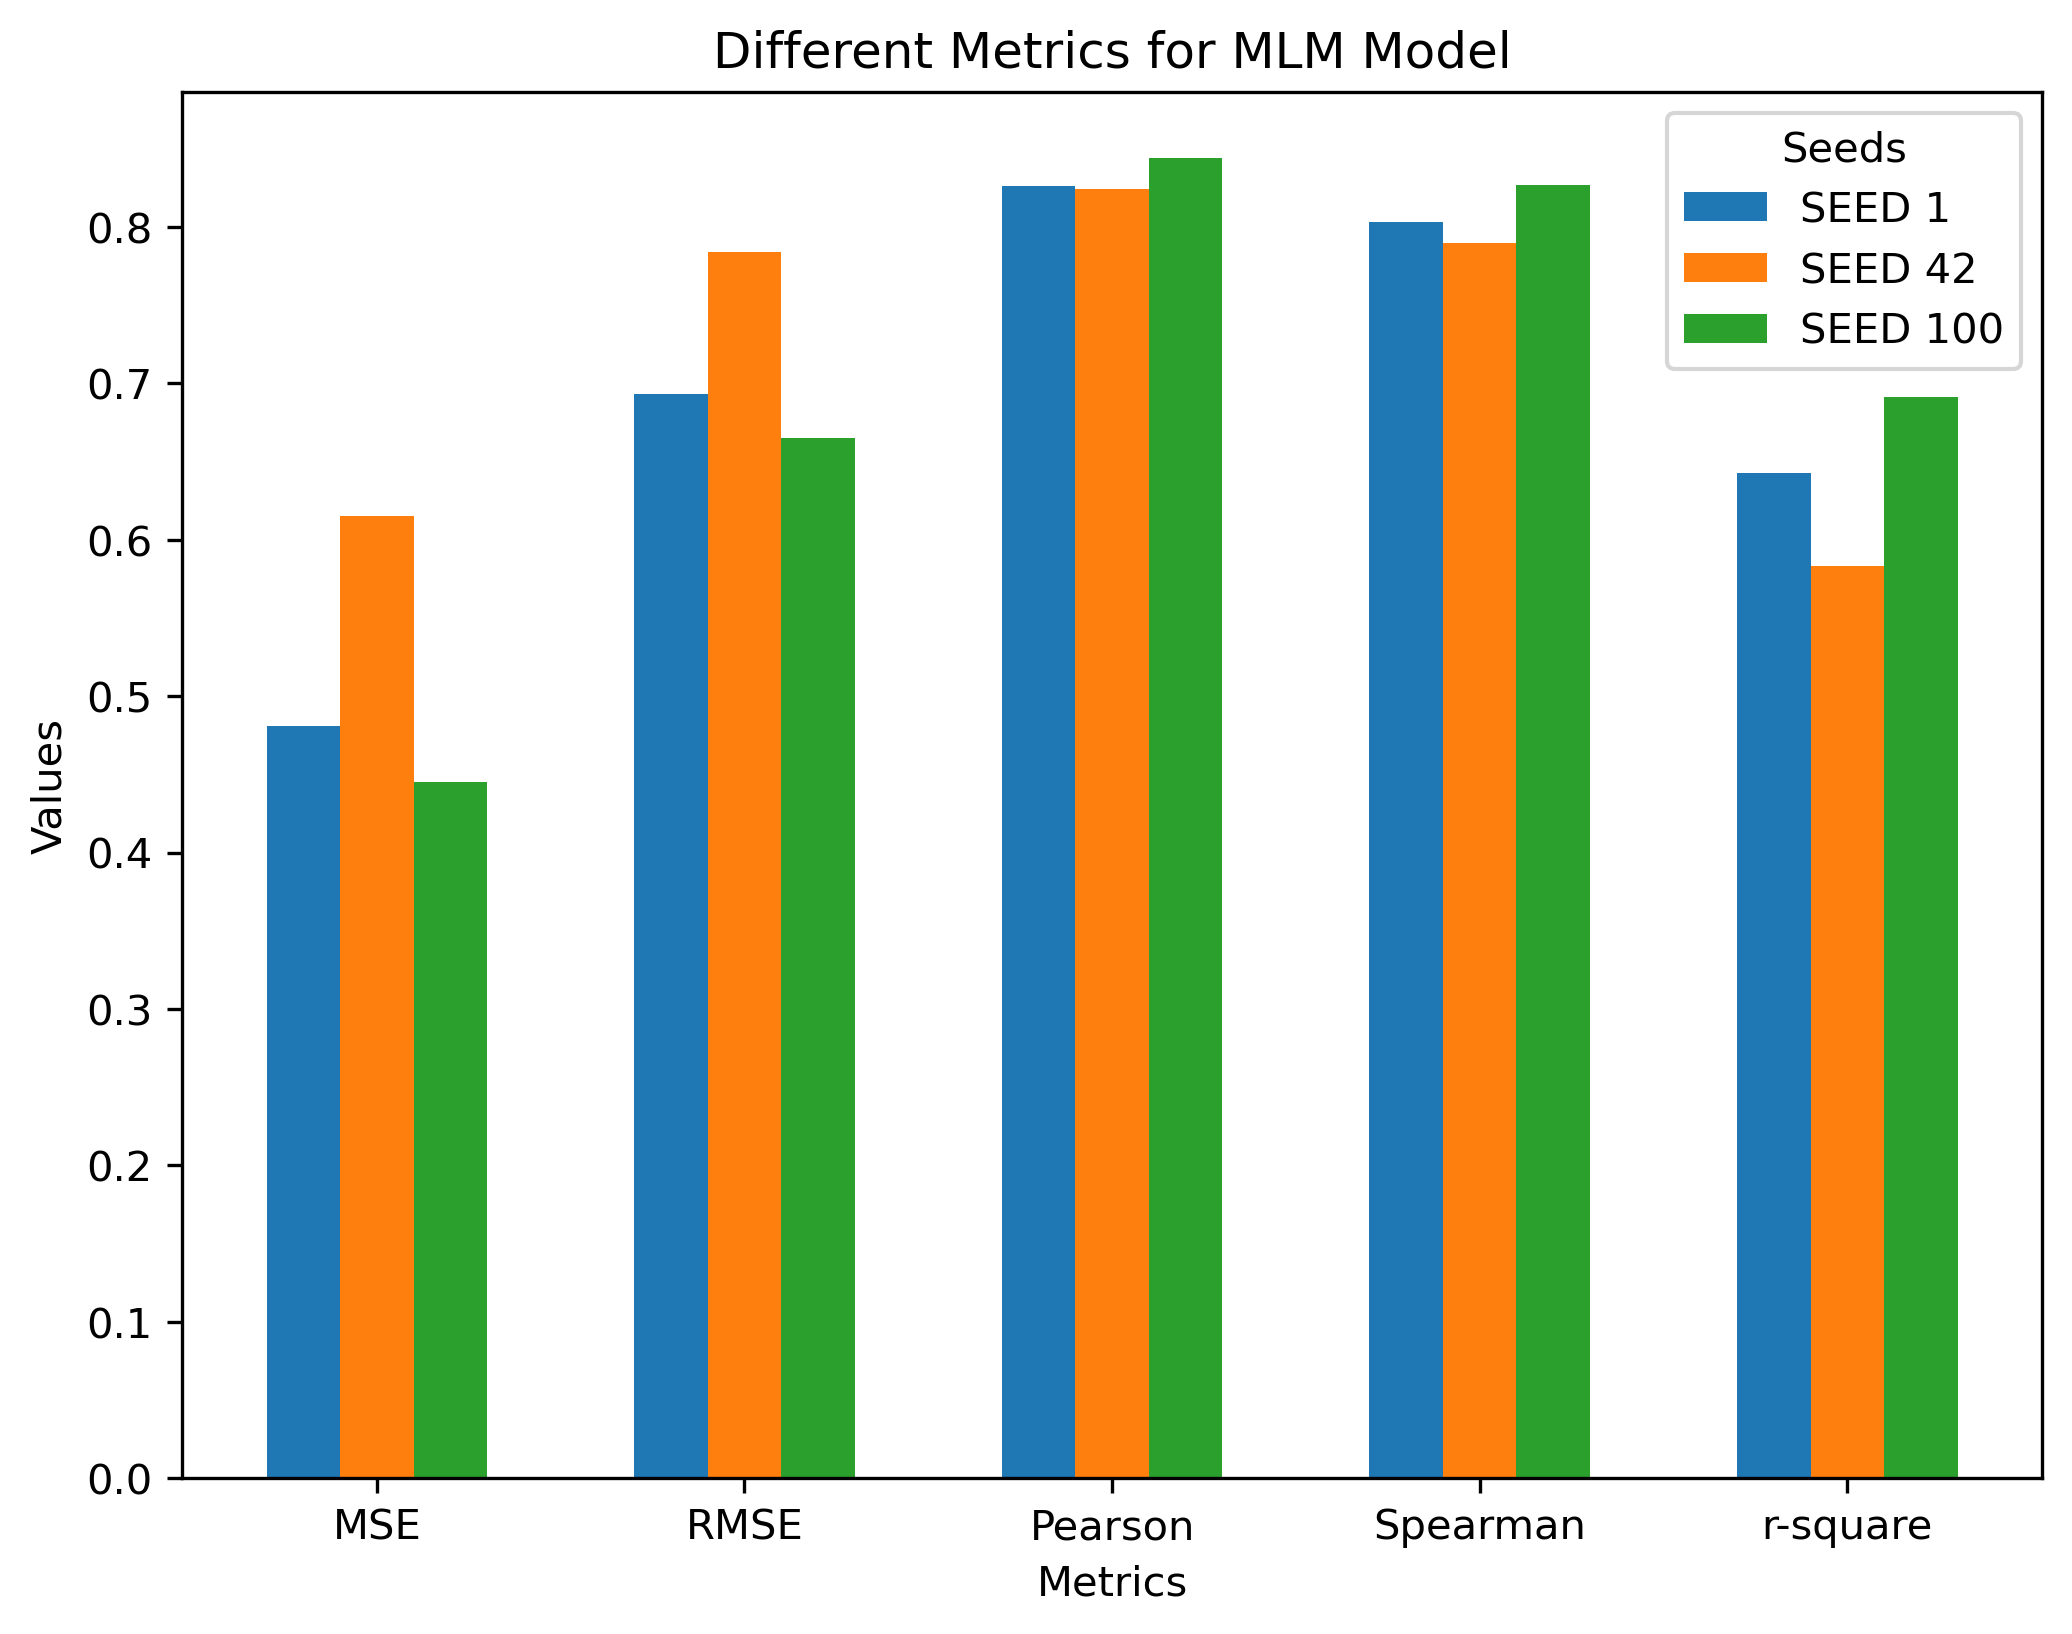
\includegraphics[width=0.5\textwidth]{pictures/mlm_model_seed.png}}
    \caption{Different performance metrics of Molformer model after masked language modeling(mlm) }
    \label{fig:mlm_seed}
\end{figure}

\section*{Influence Function-based Data Selection}

In this experiment, we incorporate both the \verb|MoleculeNet_Lipophilicity| dataset and an external dataset containing 300 samples for fine-tuning. However, unlike the straightforward inclusion approach used for \verb|MoleculeNet_Lipophilicity|, the external samples are carefully selected based on an influence function–driven procedure. 

\textbf{Influence Function} We employ influence function to determine the effect of each external sample on test set's loss function. Thus we are only selecting the most influential data points that has positive impact on model's performance. This approach follows the work of \cite{koh2020understandingblackboxpredictionsinfluence}. The influence score is formulated as:

\[
I(z) = - \nabla_{\theta} L(z_{test})^T H^{-1} \nabla_{\theta} L(z_{ext})
\]

where $I(z)$ is the influence score of an external sample $z_{ext}$, $H^{-1}$ is the approximated inverse Hessian matrix, $\nabla_{\theta} L(z)$ is the gradient of the loss function with respect to the model parameters. This is consisting of three steps-

(1) \textit{Compute gradients of test samples}- To compute gradients we use the model obtained after \verb|masked language modeling(mlm)| with regression head from task 1. Since after \verb|masked language modeling(mlm)| this model has become more domain adapted compared to the pre trained  \verb|ibm/MoLFormer-XL-both-10pct| model. 

(2) \textit{Estimate the inverse Hessian-Vector Product(iHVP)}- to compute the second-order gradient, inverse Hessian needs to be determined. However, computing the inverse of  Hessian is computationally expensive \verb|o(n^3)|. Therefore, instead of inverse Hessian, we approximate the inverse Hessian-Vector product \verb|(iHVP)| by using the LiSSA approximation (\cite{agarwal2017secondorderstochasticoptimizationmachine}).


(3)\textit{ Compute the influence score of external samples}- In order to compute the influence score, the gradients of all external samples are determined. Subsequently, we perform a \textbf{dot product} between external sample's gradient and the estimated \verb|(iHVP)|. Hence we obtain the influence score for every external samples.

\textbf{Selecting the top influential data and its impact}
After computing influence scores for 300 external samples (both positive and negative), we select the top positive samples by sorting in descending order. These high-impact samples are expected to improve model performance by reducing MSE and RMSE. We combine them with the Lipophilicity training set and fine-tune the post-masked language modeling (MLM) model with a new regression head. During testing, we compare the performance of top positive influential samples against a few samples with negative scores. The results of this analysis are shown in Figure \ref{fig:task_2_comparison}.

\begin{figure}[htp]
    \centering
    \resizebox{0.3\textwidth}{!}{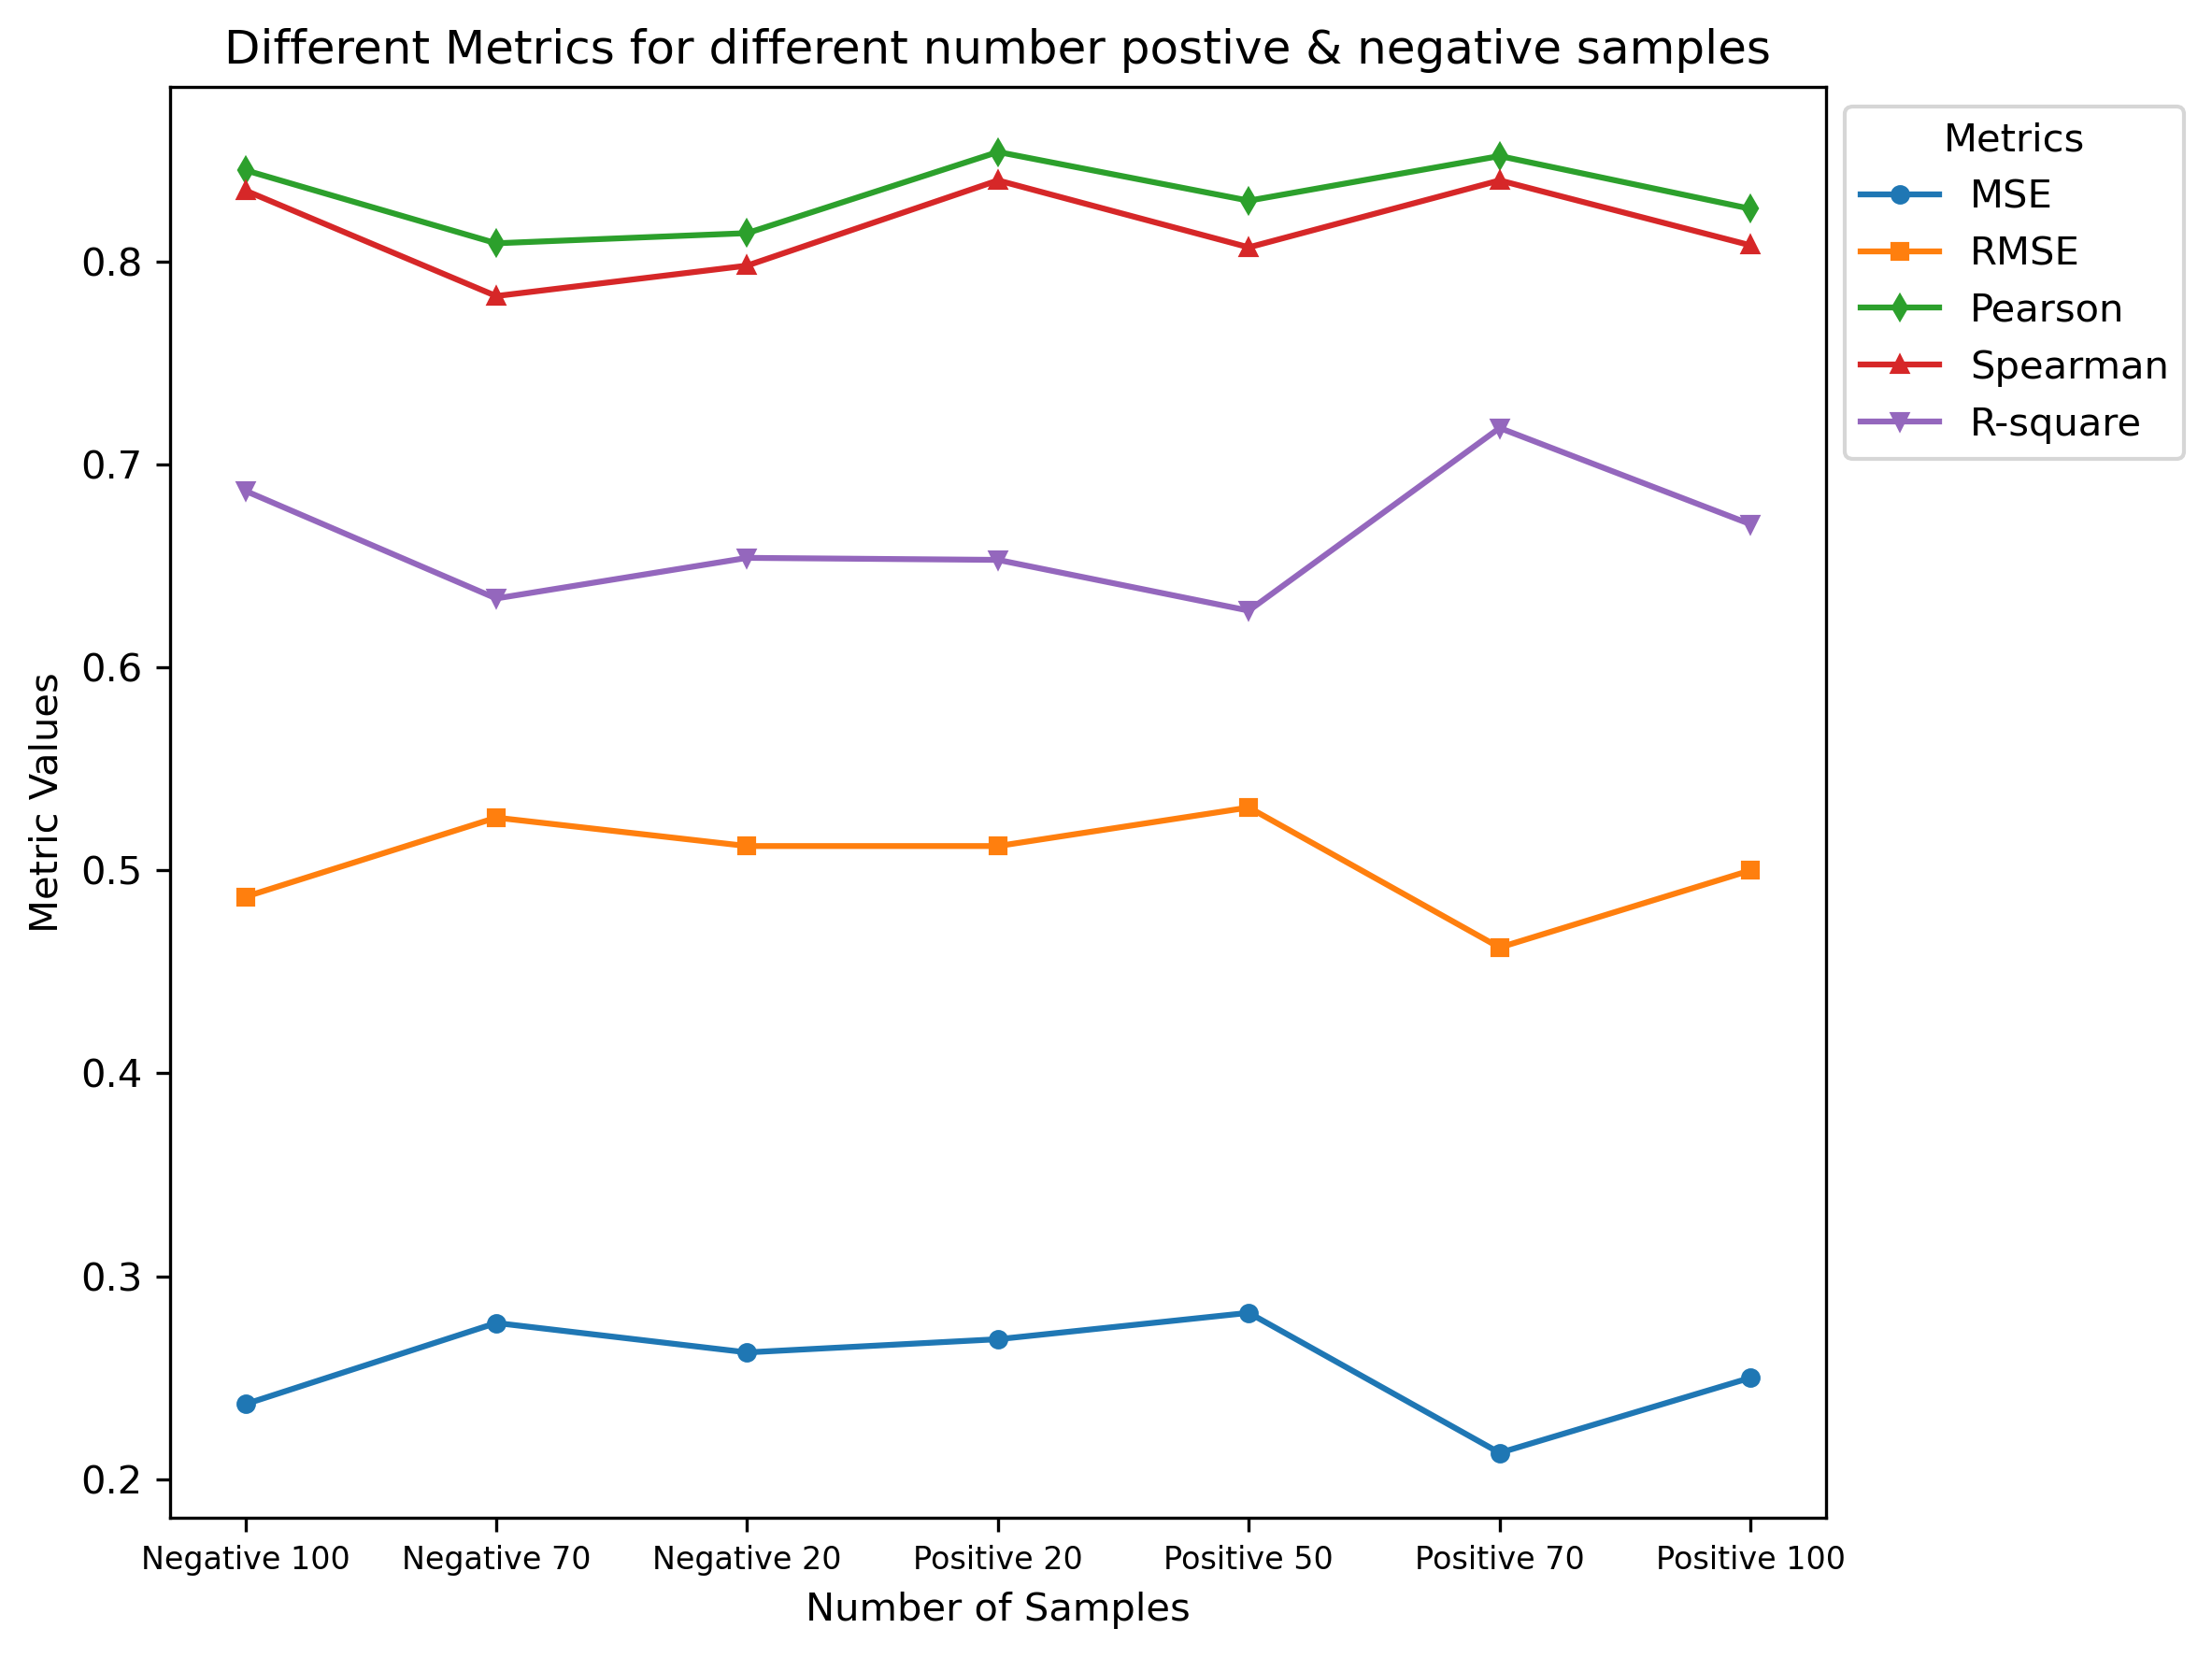
\includegraphics[width=0.5\textwidth]{pictures/task2_comparison.png}}
    \caption{Comparison of highest scored positive samples with negative scored samples }
    \label{fig:task_2_comparison}
\end{figure}

The graph analyzes sample performance across a range of sample counts: [-100, -70, -20, 20, 50, 70, 100], negative sign indicating negative influence score. Some negatively scored samples (top 100 negative) outperform even the top 50 high-scored positive samples. Among high-scored positive samples, a non-monotonic pattern emerges across all performance metrics, indicating that model performance does not consistently improve with more samples until reaching the top 70. At this point, performance improves across all metrics. One possible reason is that LiSSA, which approximates the inverse Hessian-vector product (iHVP) via an iterative algorithm, may produce deviations from the true Hessian inverse if the number of iterations or hyperparameters is not well-tuned, leading to overestimated influence scores. Additionally, external data may contain slightly different SMILES strings compared to those the model learns during mask language modeling (MLM), resulting in domain mismatch and degraded performance. Conversely, the SMILES strings within the top 70 most influential samples may be more aligned with the test data, enhancing model performance. The model trained on these top 70 samples is used for performance comparisons between Task 1 and Task 2, as illustrated in Figure \ref{fig:base_task1_task2}, with the initial fine-tuned Molformer model—prior to MLM—serving as the baseline.

\begin{figure}[t]
    \centering
    \resizebox{0.3\textwidth}{!}{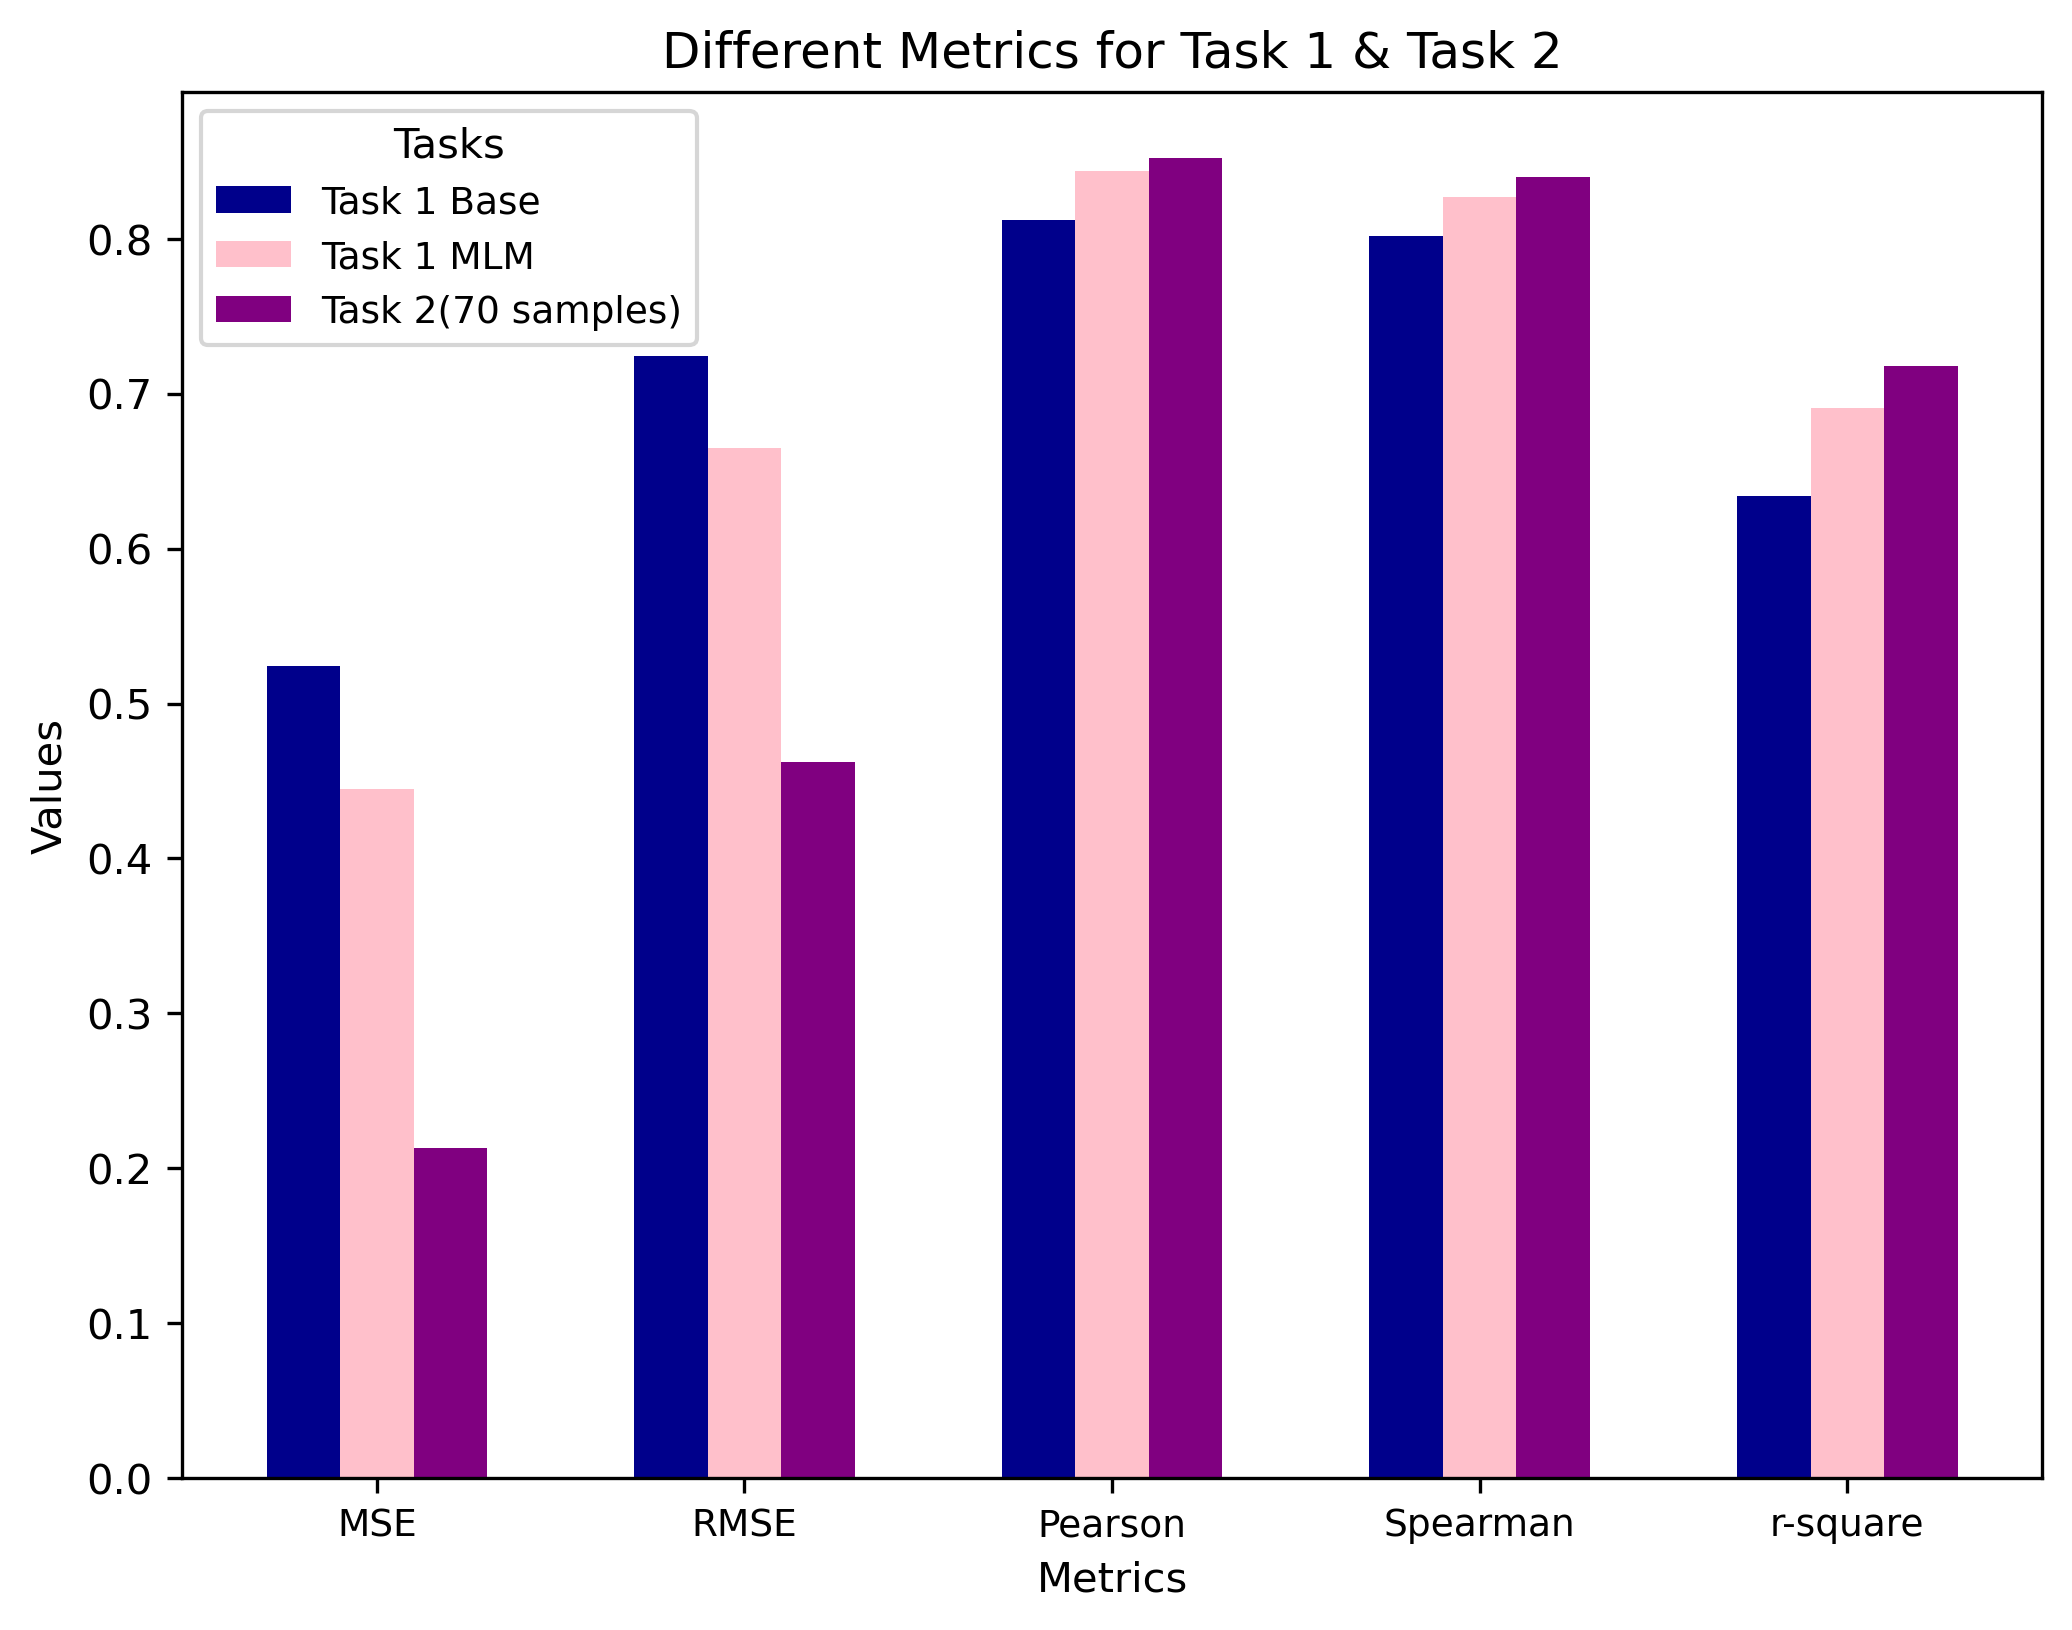
\includegraphics[width=0.5\textwidth]{pictures/base_mlm_task2_colored.png}}
    \caption{Comparison of base model, task1, task2 on performance metrics }
    \label{fig:base_task1_task2}
\end{figure}

Figure \ref{fig:base_task1_task2} shows that combination of 70 influential data with training data reveals synergic effect for all performance metrics.   

\section*{Exploration of Data Selection and Fine-Tuning Methods}

Fine-tuning a model requires careful selection of training data to ensure optimal performance. In this experiment, two data selection strategies were employed: \textbf{Diversity Sampling} and \textbf{Stratified Sampling}. The goal was to analyze how different data selection methods impact model performance and to compare the effectiveness of each strategy.

\section*{Data Selection Strategies}
\textbf{Stratified Sampling} Stratified sampling ensures that the selected data maintains the proportional distribution of different classes or features in the dataset. This method helps in reducing bias and ensuring balanced representation. The process involves (1) Binning the labels into three categories (Low, Medium, High) using quantile-based discretization (2) Performing stratified sampling to select a representative subset of data while maintaining class distribution, (3) Merging the stratified subset with the original dataset.



\textbf{Diversity Sampling} Diversity sampling ensures that selected samples are highly varied, capturing different characteristics of the dataset. This method aims to improve generalization by exposing the model to diverse patterns. The process involves (1) Generating embeddings for SMILES data using a model and tokenizer, (2) Performing diversity-based selection using clustering techniques (e.g., k-means with 5 clusters), (3) Selecting 100 diverse samples based on the generated embeddings. (4) Merging the selected dataset with the original dataset.

\begin{figure}[htp]
    \centering
    \resizebox{0.3\textwidth}{!}{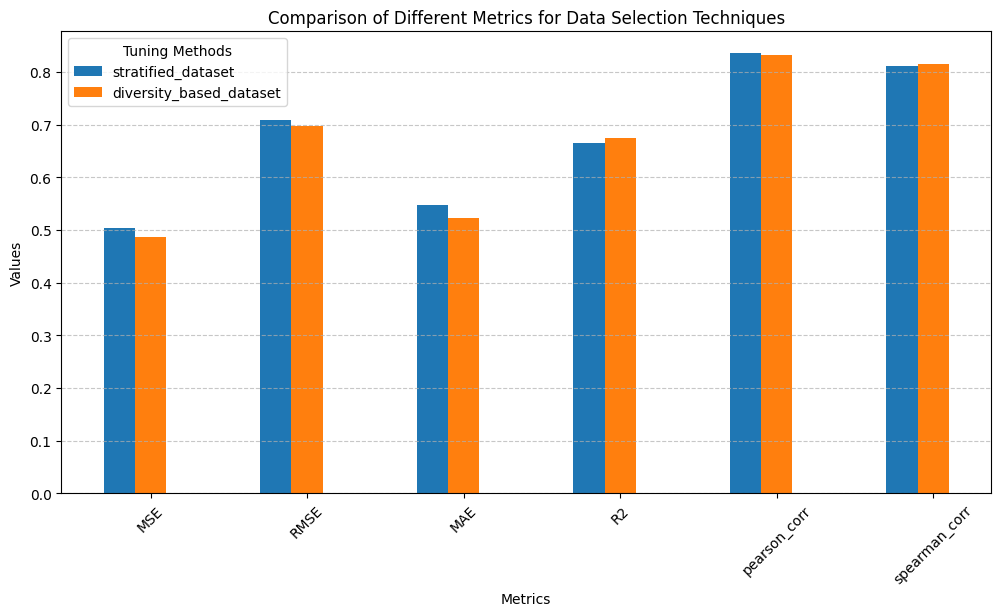
\includegraphics[width=0.5\textwidth]{pictures/data_selection_metrics_comparison.png}}
    \caption{Comparison of tuning strategies }
    \label{fig:task3a}
\end{figure}



\textbf{Analysis and Discussion}
Figure \ref{fig:task3a} summarizes the results of both data selection methods. The results indicate that, The model trained with \textbf{Diversity Sampling} achieved slightly lower error metrics (MSE: 0.4815 vs. 0.4909, RMSE: 0.6939 vs. 0.7006, MAE: 0.5129 vs. 0.5304), suggesting improved generalization. The $R^2$ score for Diversity Sampling was marginally higher (0.6801 vs. 0.6726), indicating a better fit. Pearson correlation was also higher for Diversity Sampling (0.8476 vs. 0.8371), meaning a stronger linear relationship between predicted and actual values. Spearman correlation was higher for Diversity Sampling (0.8260 vs. 0.8094), indicating a stronger rank-based association between the predictions and actual valuesOverall, \textbf{Diversity Sampling} resulted in slightly better performance, likely due to increased variety in the training data, which helped the model generalize better.


\section*{Parameter Tuning - Model Structure}
For Task 3b, we implement different algorithms to evaluate their performance on the \texttt{ibm/MoLFormer-XL-both-10pct} model. We use the \texttt{MoleculeNet\_Lipophilicity} dataset along with the external dataset provided to us for training the model.


\textbf{LoRA}(Low-Rank Adaptation) freezes pre-trained weights and introduces two low-rank matrices, \( A \) and \( B \), where \( B \in \mathbb{R}^{d \times r} \) and \( A \in \mathbb{R}^{r \times k} \). Instead of updating \( W_0 \), the model trains \( A \) and \( B \), modifying the forward pass to \( h = W_0x + BAx \). In our implementation, only the self-attention layer is replaced with LoRA, reducing trainable parameters to 885,505 (1.95\% of the total) \cite{hu2021loralowrankadaptationlarge}.

\textbf{IA3} applies learned vectors to scale model activations element-wise while keeping all parameters frozen. In self-attention, it modifies the computation as:

\[
\text{softmax}\left(\frac{Q(\mathbf{lk} \mathbf{K}^T)}{\sqrt{d_k}} (\mathbf{lv} \mathbf{V}) \right)
\]

where \( Lk \) and \( lv \) are learned vectors. Additionally, in the decoder, \( fc1 \) is scaled by another learned vector \( l_{ff} \). This introduces 295,681 new trainable parameters (0.66\% of the total) \cite{liu2022fewshotparameterefficientfinetuningbetter}.


\section*{Observation}

\begin{figure}[htp]
    \centering
    \resizebox{0.3\textwidth}{!}{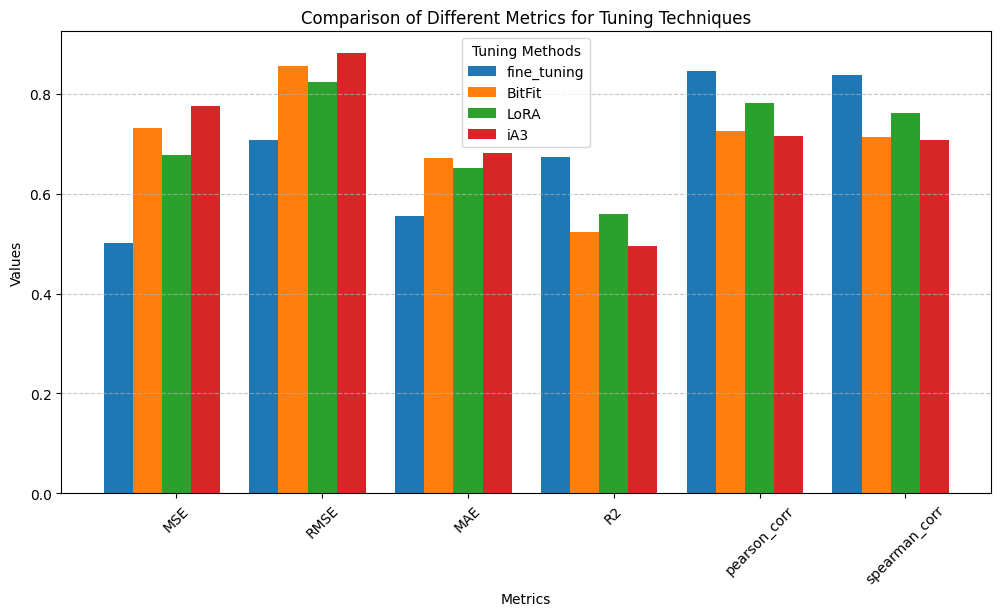
\includegraphics[width=0.5\textwidth]{pictures/tuning_metric_comparison.png}}
    \caption{Comparison of tuning strategies }
    \label{fig:task3b}
\end{figure}

\textbf{Fine Tuning} For our baseline, we first fine-tune our model. In fine-tuning, we train all the available parameters, including the model's weights and biases. For our specific model, we have 44670721 parameters. As seen in Figure~\ref{fig:task3b}, fine-tuning achieves the highest R² score (0.72), demonstrating its ability to capture the most variance. It also exhibits the lowest RMSE, confirming its strong predictive accuracy. Furthermore, fine-tuning maintains the highest Spearman correlation ensuring that predictions preserve rank relationships effectively. However, it also highlights its drawback: Fine-tuning requires the most computational resources, making it less viable for efficiency-critical applications.


\textbf{Bitfit}(bias-term fine-tuning) is a parameter-efficient tuning method that trains only the model's biases. After implementing bit fit on our current model, we are left with 370177 parameters which is just 0.82\% of the total number of parameters \cite{zaken2022bitfit}. Despite its limited parameter updates, BitFit achieves an R² score of ~0.55 (Figure~\ref{fig:task3b}), which, while lower than fine-tuning, still demonstrates competitive performance. However, it exhibits a higher RMSE, suggesting that its predictions differ more from true values. The Spearman correlation also shows a slight drop compared to fine-tuning, indicating reduced consistency in ranking relationships. BitFit, however, significantly reduces training time making it a viable option when computational efficiency is a priority.



\textbf{LoRA} emerges as the best alternative to fine-tuning, striking a balance between accuracy and efficiency. LoRA achieves an R² score of ~0.65 (Figure~\ref{fig:task3b}), closely approaching fine-tuning. Its RMSE remains lower than that of BitFit and iA3, strengthening its predictive strength. Furthermore, we see that LoRA maintains a high Spearman correlation, preserving relative rankings within the data. While its training time is comparable to fine-tuning, the reduction in trainable parameters makes it more computationally efficient. This adaptability makes LoRA a strong contender for real-world applications requiring both performance and efficiency.

\textbf{IA3} Among all techniques, iA3 exhibits the most significant increase in error rates. As seen in Figure~\ref{fig:task3a}, iA3 achieves the lowest R² score (~0.50), meaning it explains the least variance in the data. Its RMSE is the highest among all techniques, confirming that its predictions are more prone to deviations. It also indicates that iA3 has the lowest Spearman correlation, suggesting that it struggles to maintain rank-based relationships. However, the key advantage of iA3 lies in its efficiency as it has the shortest training time, making it a suitable option for scenarios where computational resources are limited.

\section*{Conclusion} 

In this study, we perform fine-tuning and masked language modeling on chemical LM. We observe that combination of training set with influential samples selected based on influence score significantly improves performance. Though influence score should be determined with caution as it can be overestimated, adversely effecting model's performance. Diversity Sampling showed slight performance improvements over Stratified Sampling. We found that BitFit offers efficiency gains but struggles with generalization, while iA3 prioritizes training speed at the expense of predictive quality.  Maintaining strong accuracy while reducing trainable  parameters, LoRA might be the most practical alternative to full model fine-tuning. As future work, we should explore more powerful parameter and computation efficient fine-tuning techniques and explore hybrid data selection strategies to improve models overall efficiency and performance. 
 

% Entries for the entire Anthology, followed by custom entries
% \bibliography{anthology,custom}
% \bibliographystyle{acl_natbib}
% \bibliographystyle{acl_natbib} % Use the ACL citation style
% \bibliography{custom} % Ensure "custom.bib" is the correct filename
\bibliography{anthology,custom}
\bibliographystyle{acl_natbib}
% \bibliographystyle{acl_natbib}
% \bibliography{references}
% \appendix

% \section{Example Appendix}
% \label{sec:appendix}

% This is a section in the appendix.

\end{document}

